\begin{activity} \label{A:9.7.8} The left side of figure
  \ref{F:9.7.space.curve} shows the curve described by the
  vector-valued function
  $$\vr(t) = \left\langle 2t-\frac12 t^2 + 1,
        t-1\right\rangle.$$

\begin{figure}[ht]
  \begin{center}
    \includegraphics{figures/fig_9_7_space_curve.eps}
    \hspace*{20pt}
    \includegraphics{figures/fig_9_7_speed_graph.eps}
    \caption{The curve $\vr(t) = \left\langle 2t-\frac12 t^2 + 1,
        t-1\right\rangle$ and its speed.}
    \label{F:9.7.space.curve}
  \end{center}
\end{figure}

\ba
\item Find the object's velocity $\vv(t)$.

\item Find the object's acceleration $\va(t)$.

\item Indicate on the left of Figure \ref{F:9.7.space.curve} the object's
  position, velocity and acceleration at the times $t=0, 2, 4$.  Draw
  the velocity and acceleration vectors with their tails placed at the
  object's position.

\item Recall that the speed is $|\vv| = \sqrt{\vv\cdot\vv}$. Find the object's speed and graph it as a function of time $t$ on the right of Figure \ref{F:9.7.space.curve}.  When is the
  object's speed the slowest?  When is the speed increasing?  When it
  is decreasing?

\item What seems to be true about the angle between $\vv$ and $\va$ when the speed
  is at a minimum?  What is the angle between $\vv$ and $\va$
  when the speed is increasing?  when the speed is decreasing?

\item   Since the square root is an increasing function, we see that the speed
  increases precisely when $\vv\cdot\vv$ is increasing.  Use the
  product rule for the dot product to express
  $\frac{d}{dt}(\vv\cdot\vv)$ in terms of the velocity $\vv$ and
  acceleration $\va$.  Use this to explain why the speed is increasing
  when $\vv\cdot\va > 0$ and decreasing when
  $\vv\cdot\va < 0$. Compare this to part (d). 

\item Show that the speed's rate of change is
  $$
  \frac{d}{dt}|\vv(t)| = \comp_{\vv} \va.
  $$





\ea

\end{activity}
\begin{smallhint}

\end{smallhint}
\begin{bighint}

\end{bighint}
\begin{activitySolution}
   \ba
    \item Velocity is the derivative of position, so
\[\vv(t) = \vr'(t)= \langle 2-t, 1 \rangle.\]


    \item Acceleration is the derivative of velocity, so
\[\va(t) = \vv'(t)= \langle -1, 0 \rangle.\]

    \item Notice that $\vr(0) = \langle 1,-1 \rangle$, $\vr(2) = \langle 2,1 \rangle$, and $\vr(4) = \langle 0,3 \rangle$. The vectors at each point are shown in the figure below at left. 


    \item Speed is the magnitude of the velocity, so the speed of the object at time $t$ is
\[s(t) = \sqrt{(2-t)^2+1}.\]
The speed of the object is at its least when $t=2$. The speed is increasing on the interval $(2,4)$ and decreasing on the interval $(-4,2)$.  
\begin{center}
\resizebox{!}{2.5in}{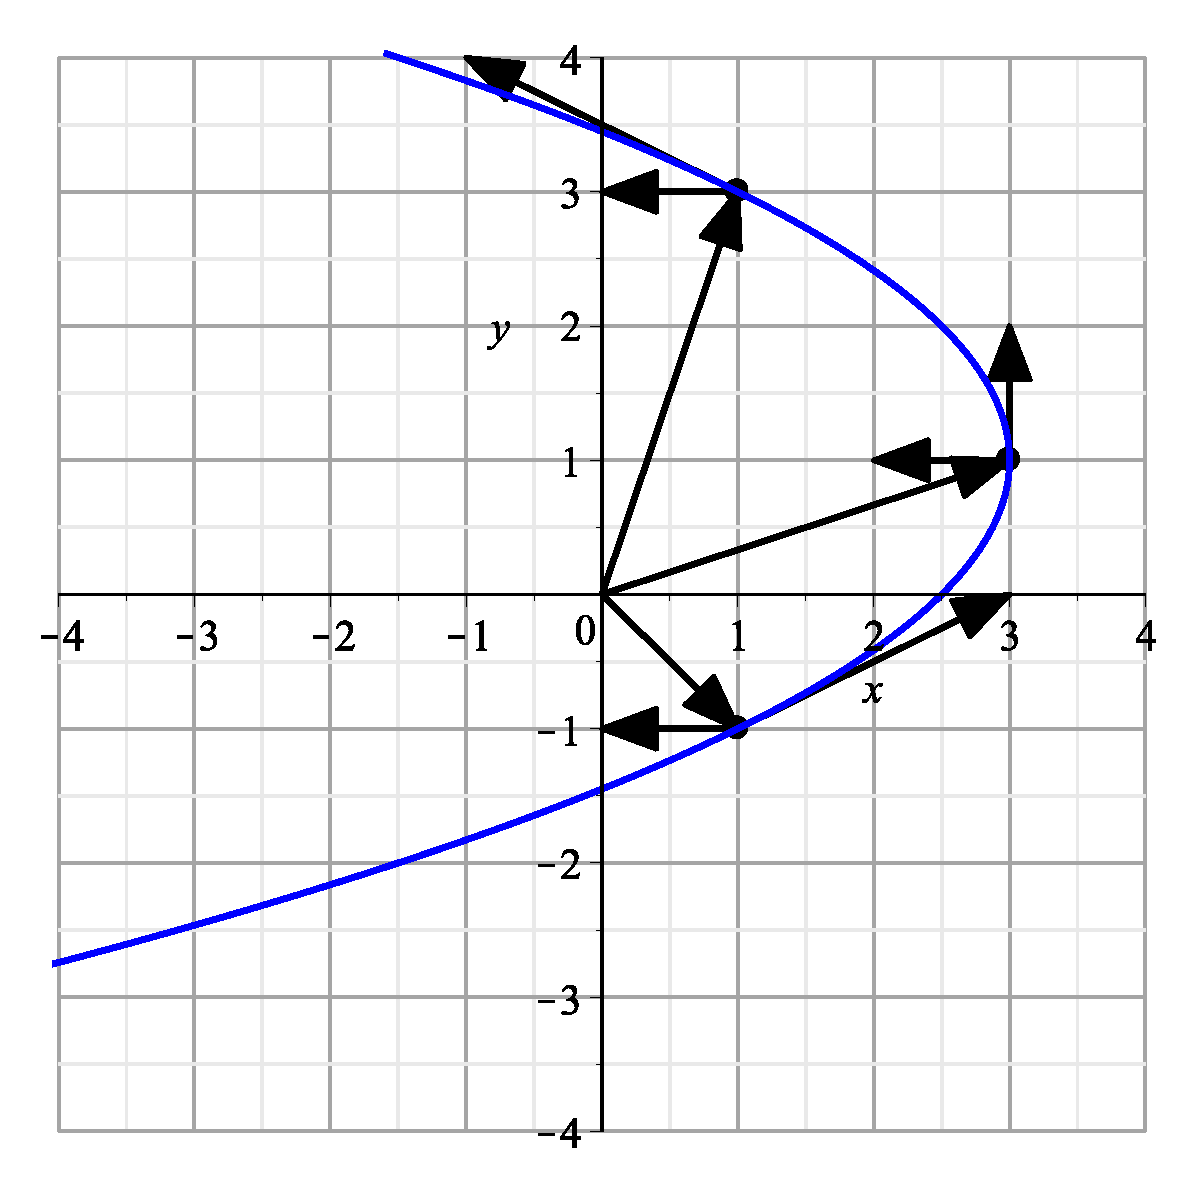
\includegraphics{figures/9_7_8_a.eps}} \ \ \ \  \resizebox{!}{2.5in}{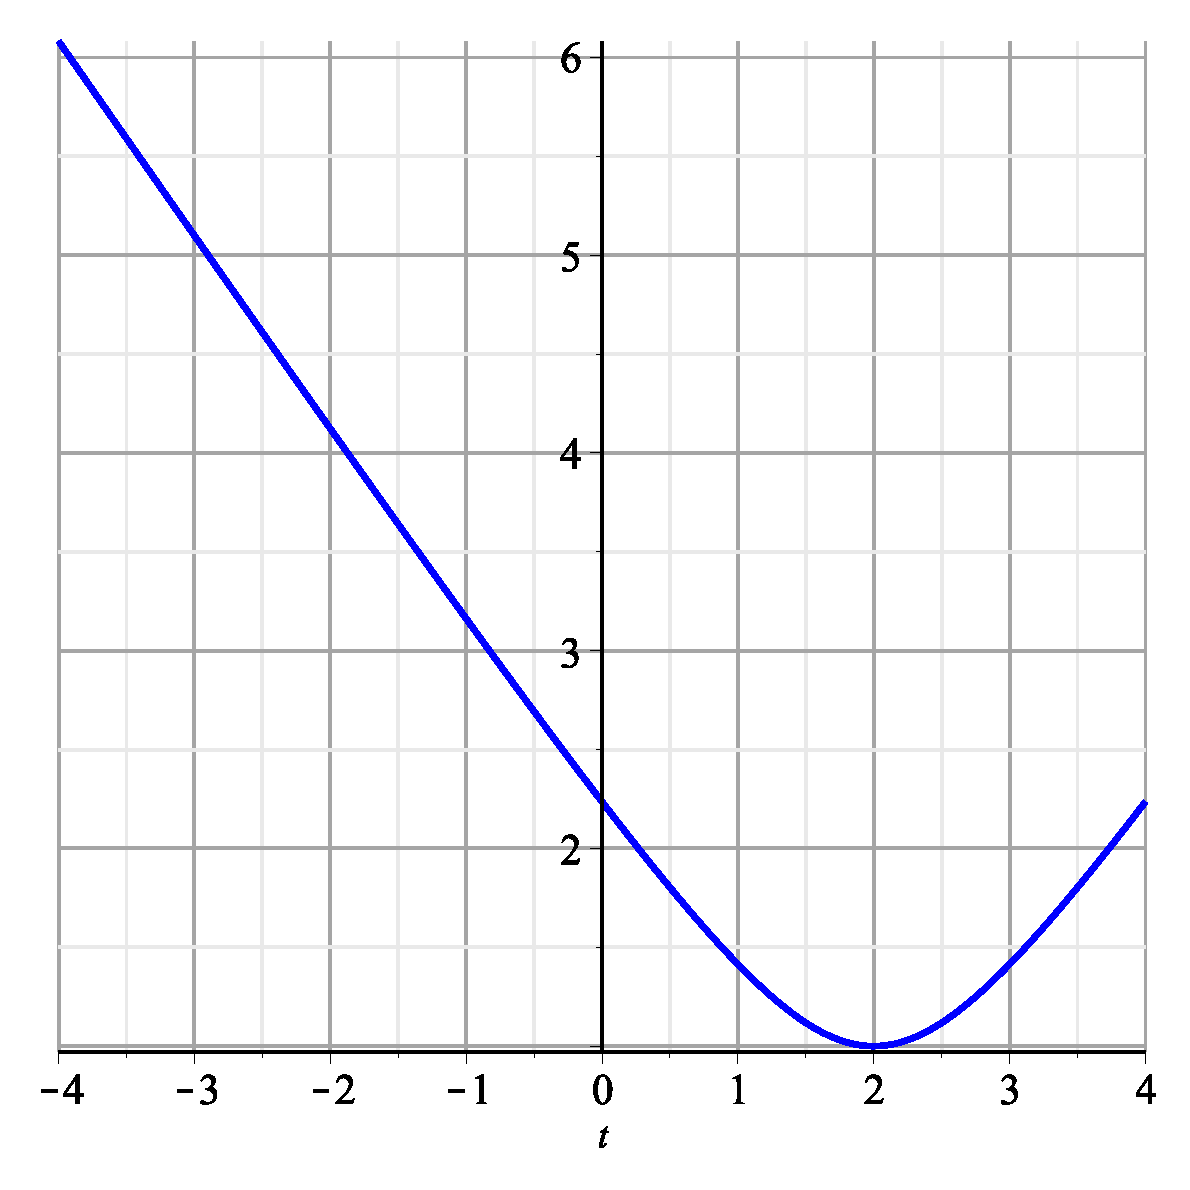
\includegraphics{figures/9_7_8_b.eps}}
\end{center}

\item When $t < 2$ in the position graph, the angle between $\vv$ and $\va$ is larger than $90^{\circ}$. When $t > 2$ in the position graph, the angle between $\vv$ and $\va$ is less than $90^{\circ}$. Note that at the point when $t=2$, the vectors $\vv$ and $\va$ are orthogonal.

	\item Using derivative properties we have 
	\[\frac{d}{dt}(\vv\cdot\vv) = \vv \cdot \frac{d}{dt} \vv + \frac{d}{dt} \vv \cdot \vv = 2(\vv \cdot \va).\]
	So the derivative of the speed is positive when $\vv \cdot \va$ is positive and negative when $\vv \cdot \va$ is negative. In other words, speed is increasing when $\vv \cdot \va$ is positive and decreasing when $\vv \cdot \va$ is negative. When $t < 2$ in the position graph, the angle between $\vv$ and $\va$ is larger than $90^{\circ}$ and so $\vv \cdot \va < 0$. When $t > 2$ in the position graph, the angle between $\vv$ and $\va$ is less than $90^{\circ}$ and so $\vv \cdot \va > 0$. Note that at the point when $t=2$, the vectors $\vv$ and $\va$ are orthogonal.  

\item In general, if $\vr(t) = \langle x(t), y(t) \rangle$, then $\vv(t) = \langle x'(t), y'(t) \rangle$, $\va(t) = \langle x''(t), y''(t) \rangle$, and the speed is $s(t) = \sqrt{(x'(t))^2 + (y'(t))^2}$. Recall that $\comp_{\vv} \va = \frac{\va \cdot \vv}{|\vv|}$, so
\[\frac{d}{dt} s(t) = \frac{x'(t)x''(t) +y'(t)y''(t)}{|\vv|} = \comp_{\vv} \va.\]
 

   \ea

\end{activitySolution}
\aftera
